\documentclass[usenames,dvipsnames,aspectratio=169]{beamer}
\usepackage[utf8]{inputenc}
\usecolortheme{seahorse}
\usepackage{amsmath,xfrac,dsfont,amsfonts,bbm,cancel,euler,ulem}
\usepackage{apacite,natbib}
\usepackage{hyperref}
\usepackage{caption,subcaption,booktabs,multicol,adjustbox}
\usepackage{xcolor,enumitem}

\setbeamercolor{section in toc}{fg=violet}
\setbeamercolor{subsection in toc}{fg=violet}

\title{The Missing ``Missing Middle'' \\ \small{Applied Macroeconomics: Micro Data for Macro Models} }
\author{Author: Chang-Tai Hsieh \and Benjamin A. Olken \\ Presented by: Jose M. Quintero}

\newcommand{\thus}{$\textcolor{violet}{\Longrightarrow}$}

\AtBeginSection[]
{
  \begin{frame}<beamer>
    \frametitle{Outline}
    \tableofcontents[currentsection]
  \end{frame}
}

\AtBeginSubsection[]
{
   \begin{frame}
        \frametitle{Outline}
        \tableofcontents[currentsubsection]
   \end{frame}
}



\begin{document}

\begin{frame}
  \titlepage
\end{frame}

\begin{frame}{Motivation}
    \begin{itemize}[label=\textcolor{violet}{$\blacktriangleright$}]
        \item \underline{The Missing Middle}: Few medium-size firms in developing countries relative to small and large firms. 
        \vfill
        \item Two prevailing theories:
        \begin{enumerate}[label=\textbf{\textcolor{violet}{\arabic*.}}]
            \item Small firms are disfavor by institutional setting $\textcolor{violet}{\Longrightarrow}$ Hard for small firms to grow.
            \item The burden of regulation is heavier on big firms $\textcolor{violet}{\Longrightarrow}$ Only very productive firms can overcome regulations. 
        \end{enumerate}
        \vfill 
        \item This Paper: Challenges the existence ``Missing Middle.''
        \begin{enumerate}[label=\textbf{\textcolor{violet}{\arabic*.}}]
            \item Test the implications of existing theories using Micro-data
            \item Why do we observe the ``Missing Middle''? 
        \end{enumerate}     
    \end{itemize}
\end{frame}

\begin{frame}{Main Results}
    \begin{enumerate}[label=\textbf{\textcolor{violet}{\arabic*.}}]
        \item There is no ``Missing Middle'' in the firm size distribution
        \begin{itemize}[label=\textcolor{violet}{$\blacktriangleright$}]
            \item Firm size distribution is not bimodal $\textcolor{violet}{\Longrightarrow}$ Big firms are also absent.
            \item Employment share \textcolor{violet}{+} Binning $\textcolor{violet}{\Longrightarrow}$ The ``Missing Middle'' 
            \item Size-dependent distortions barely generate bunching. 
        \end{itemize}
        \vfill
        \item Microdata does not favor constrained small firms:
        \begin{itemize}[label=\textcolor{violet}{$\blacktriangleright$}]
            \item No bimodality in the distribution of average return to inputs. 
            \item Marginal return to capital is higher for larger firms. 
        \end{itemize}            
        \vfill
        \item Data favors that the burden of regulation is heavier on big firms
        \begin{itemize}[label=\textcolor{violet}{$\blacktriangleright$}]
            \item Results may vary upon underlying technology assumption. 
        \end{itemize}
    \end{enumerate}
\end{frame}

\section{Existing Theories}

\begin{frame}{Disfavored Small Firms}
    \begin{itemize}[label=\textcolor{violet}{$\blacktriangleright$}]
        \item Institutional setting disfavor small firms. 
        \begin{itemize}[label=\textcolor{violet}{\small{$\blacktriangleright$}}]
            \item Credit constrained, financial access,
            \item Property rights are better protected for formal, 
            \item Policies favor big firms. 
        \end{itemize}
        \vfill
        \item Empirical Predictions
        \begin{enumerate}[label=\textbf{\textcolor{violet}{\arabic*.}}]
            \item Small and big firms are unconstrained \thus Marginal return to inputs is low. 
            \item ``Missing'' mid-size firms are constrained \thus Marginal return to inputs are high. 
            \item Bimodal distribution of marginal returns to inputs. 
        \end{enumerate}
    \end{itemize}
\end{frame}

\begin{frame}{A Dual Economy}
    \begin{itemize}[label=\textcolor{violet}{$\blacktriangleright$}]
        \item Medium and large firms face costs that small firms do not face. 
        \begin{enumerate}[label=\textbf{\textcolor{violet}{\arabic*.}}]
            \item Mid-size firms cannot overcome the barriers \thus Remain small. 
            \item Ej: Size-dependent regulations, minimum wages, registration (fix costs). 
        \end{enumerate}
        \vfill
        \item Empirical Predictions
        \begin{enumerate}[label=\textbf{\textcolor{violet}{\arabic*.}}]
            \item Barbell shaped for returns to capital. 
            \item Returns to inputs by firm size are dependent on production technology. 
            \item Size-dependent distortions \thus Right skewed f.s.d + higher return for big firms. 
        \end{enumerate}
    \end{itemize}
\end{frame}

\section{Testing against the data}
\begin{frame}{Firm Size Distribution}
    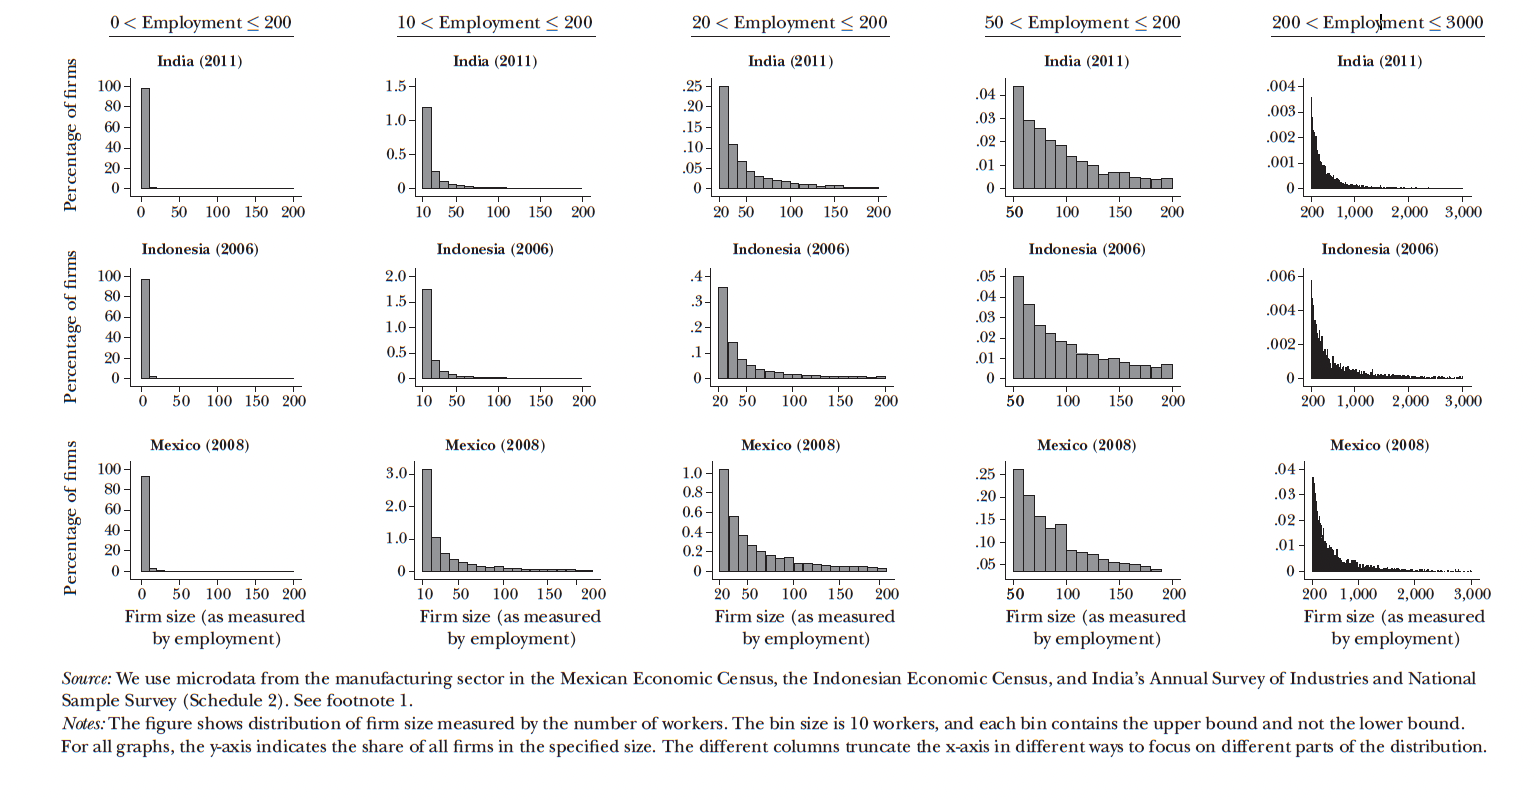
\includegraphics[width=\textwidth]{Figures/FirmSizeDist.png}
\end{frame}

\begin{frame}{Distribution of Average products}
\begin{center}
    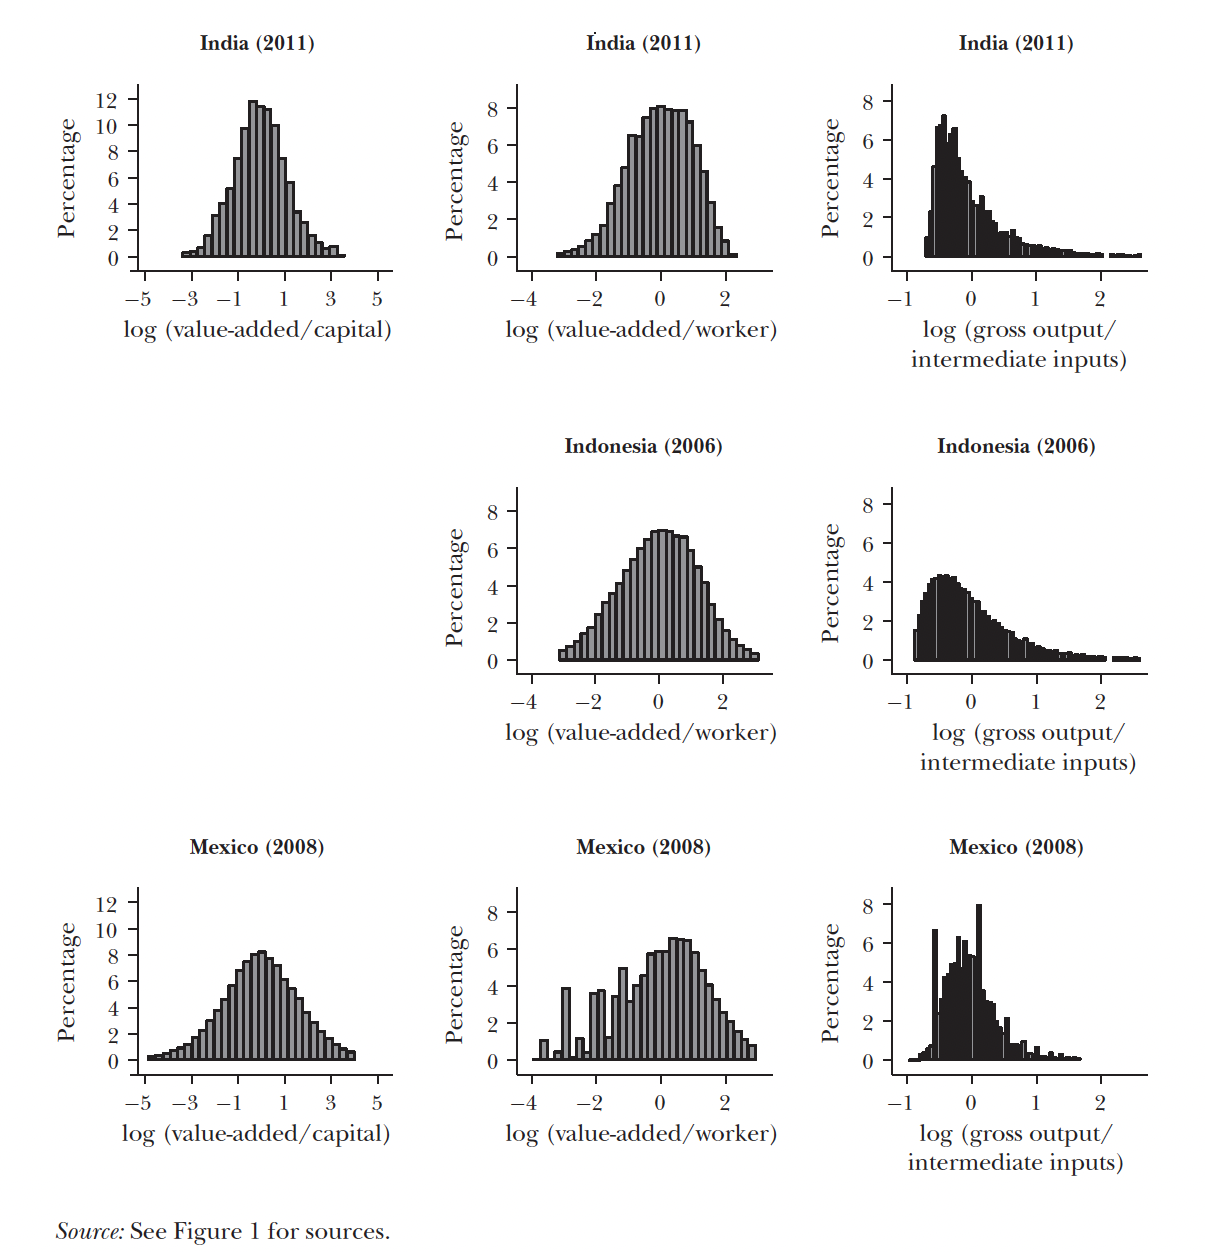
\includegraphics[width=0.55\textwidth]{Figures/ReturnDistribution.png}
\end{center}
\end{frame}

\begin{frame}{Size-Dependent Distortions}
    \begin{enumerate}[label=\textbf{\textcolor{violet}{\arabic*.}}]
        \item Distortion in terms of employment
        \begin{itemize}[label=\textcolor{violet}{$\blacktriangleright$}]
            \item India: Firms over 100 workers have firing costs.
        \end{itemize}
        \vfill
        \item Distortions in terms of revenue
        \begin{itemize}[label=\textcolor{violet}{$\blacktriangleright$}]
            \item Mexico: Discontinuous change in tax rates after threshold. 
            \item Indonesia: Firms below threshold exempt from 10\% VAT.
        \end{itemize}
    \end{enumerate}
\end{frame}

\begin{frame}{The case of Mexico}
\begin{center}
    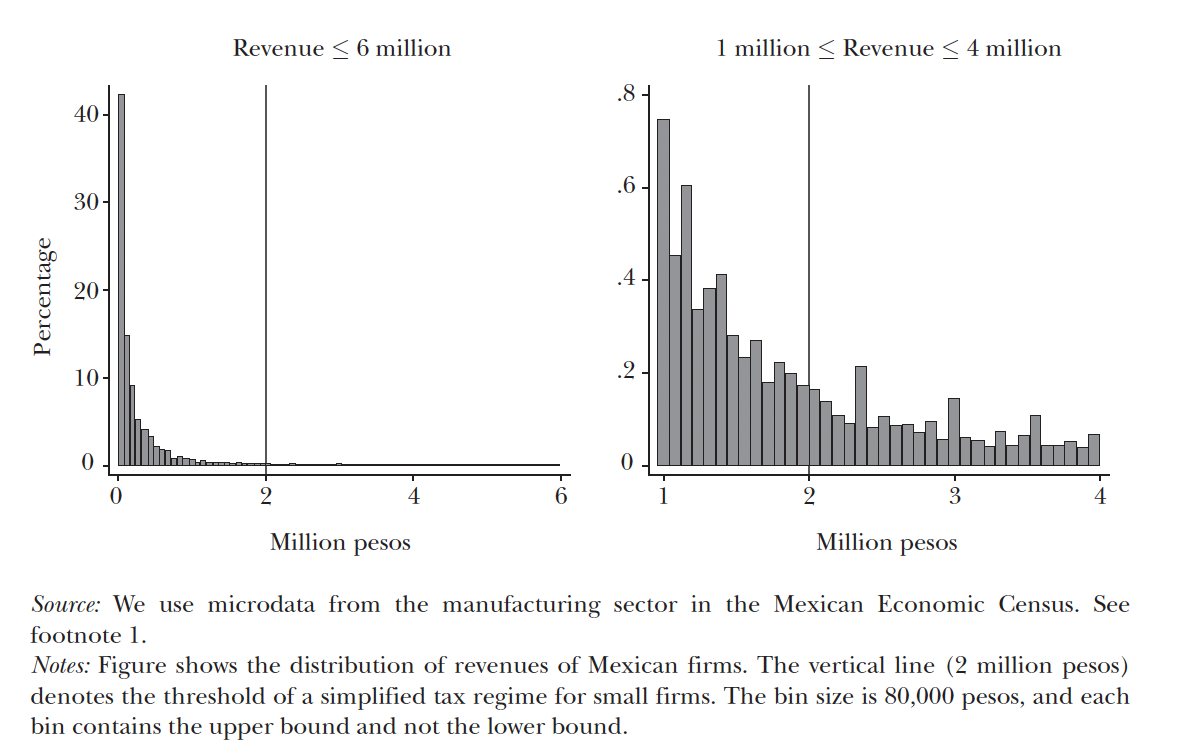
\includegraphics[width=0.8\textwidth]{Figures/MexicoSizeDependent.png}
\end{center}
\end{frame}

\begin{frame}{The Case of India}{Informality}
\begin{center}
    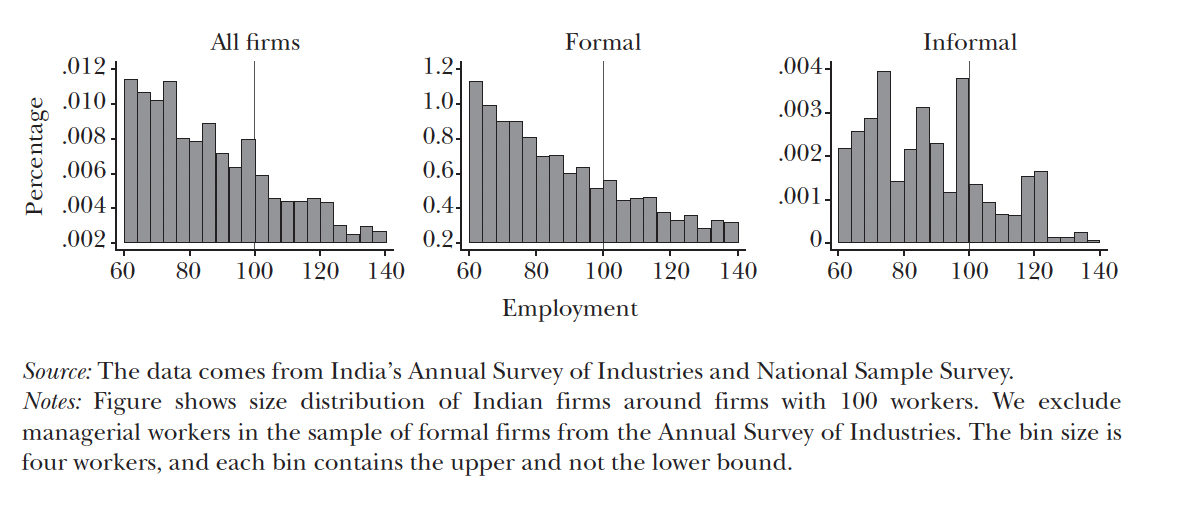
\includegraphics[width=\textwidth]{Figures/IndiaSizeDependent.png}
\end{center}
\end{frame}

\section{Missing Middle Origin}

\begin{frame}{Employment Share vs Firm Size Dist}
\begin{itemize}[label=\textcolor{violet}{$\blacktriangleright$}]
    \item Previous papers: Study the employment share distribution by firm size
    \begin{equation*}
        \text{Employment Share}(n) = \dfrac{n\times\#\text{Firms}(n)}{\text{Total Employment}}\neq  \dfrac{\#\text{Firms}(n)}{\text{Total Firms}}
    \end{equation*}
    \vfill
    \pause
    \item Ej: 100 workers, 10 Firms
    \begin{center}
    \small{
        \begin{tabular}{cccc} \hline\hline
            \# Firms & \# Workers & \% Firms & \% Workers \\ \hline
                1 &  40 & 10\% & 40\% \\ 
                1 &  20 & 10\% & \textcolor{red}{20\%} \\ 
                8 &  5  & 80\% & 40\% \\ 
                \hline\hline
        \end{tabular}
        }
    \end{center}
\end{itemize}
\end{frame}

\begin{frame}{Taking it to the data}
\begin{table}[h]
    \begin{center}
    \begin{tabular}{lccc}
    \hline \hline
    Firm Size (Employment) & India 2011 & Indonesia 2006 & Mexico 2008 \\
    \hline 
    \multicolumn{4}{l}{\textit{Panel A: Distribution of Firm Size}} \\
    $1-9$ & $97.88$ & $96.78$ & $91.74$ \\
    $10-49$ & $1.85$ & $2.83$ & $5.85$ \\
    $50+$ & $0.28$ & $0.39$ & $2.41$ \\
    & & & \\
    \multicolumn{4}{l}{\textit{Panel B: Distribution of Employment Share by Firm Size}} \\
    $1-9$ & $64.77$ & $53.95$ & $22.45$ \\
    $10-49$ & $12.10$ & $12.04$ & $10.55$ \\
    $50+$ & $23.13$ & $34.01$ & $66.99$ \\
    \hline\hline
    \end{tabular}
    \end{center}
    \footnotesize{Source: See Figure 1 for sources.}
    \end{table}
\end{frame}

\begin{frame}{Conclusions}
    \begin{itemize}[label=\textcolor{violet}{$\blacktriangleright$}]
        \item There is no ``Missing'' Middle. 
        \begin{enumerate}[label=\textbf{\textcolor{violet}{\arabic*.}}]
            \item It arises from employment share distribution, 
            \item Big firms are also absent \thus Very skewed f.s.d. 
        \end{enumerate}
        \vfill
        \item Microdata does not favor existing theories:
        \begin{enumerate}[label=\textbf{\textcolor{violet}{\arabic*.}}]
            \item The simplest form of small firm constrained and dual economy are not consistent with empirics. 
            \item Data leans towards big firms begin constrained. 
            \item Policies targetted to favor small firms increase incentives to stay small. 
        \end{enumerate}
    \end{itemize} 
\end{frame}


\begin{frame}{Average Product and Firm Size}
\begin{center}
    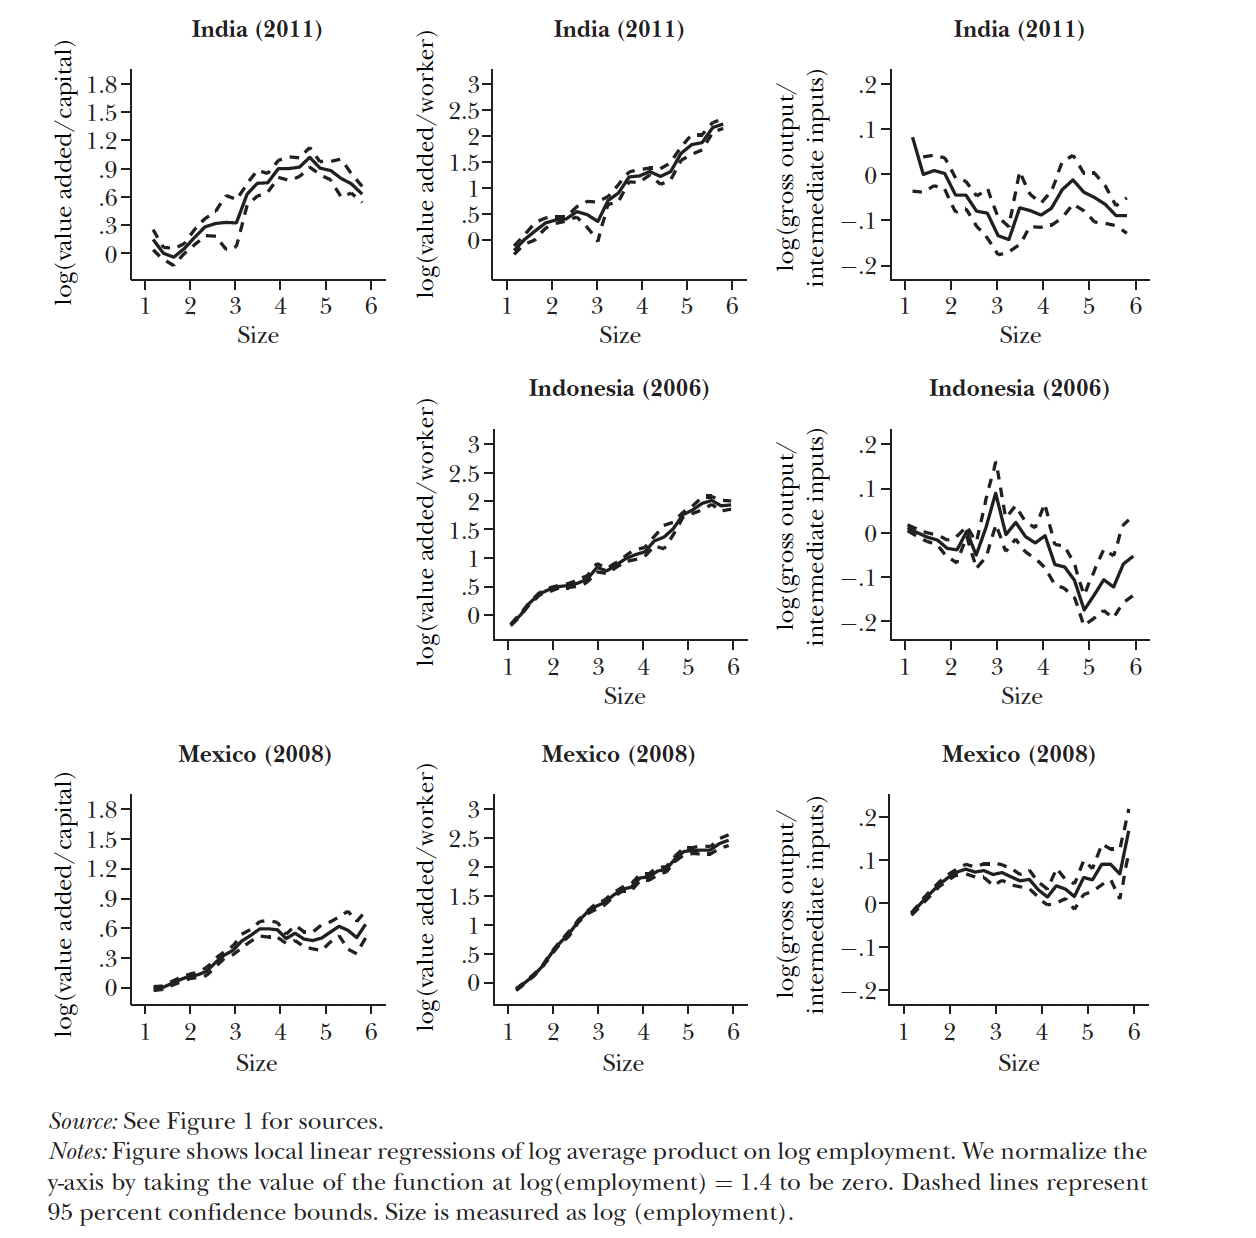
\includegraphics[width=0.65\textwidth]{Figures/ReturnFirmSize.png}
\end{center}
\end{frame}

\end{document}

